\documentclass[titlepage]{article}
\usepackage[PunctStyle=banjiao]{xeCJK}
\setCJKsansfont{Noto Sans CJK SC}
\setCJKmainfont{Noto Serif CJK SC}
\setCJKmathfont{Noto Serif CJK SC}
\usepackage{indentfirst}
\setlength{\parindent}{2em}
\usepackage{enumitem}
\usepackage{amsmath}
\usepackage{graphicx}
\usepackage{float}
\usepackage{wrapfig}
\usepackage[export]{adjustbox}
\usepackage{xcolor}
\usepackage{ulem}
\usepackage{CJKfntef}
\newcommand{\passthrough}[1]{#1}
\usepackage{hyperref}
\hypersetup{
	colorlinks=true,
	linkcolor=cyan,
	filecolor=cyan,      
	urlcolor=cyan,
	citecolor=cyan,
}
\usepackage[margin=0.2cm]{geometry}


\title{{
\includegraphics[scale=0.3]{gnulinux-logo.png}}\\ {GNU/Linux for daily use}}
\author{spinach/hehelego}
\date{\today}

\begin{document}
\maketitle

\section*{这是什么}


\noindent \sout{Linux日常使用、开发环境、服务维护的相关教程、书籍、博客等资料已经非常多了}\\[0pt] \sout{遍地都是,随便一搜就是一大把.不要给geekpie workshop灌水啊}\\

这是一个关于GNU/Linux OS的基本介绍,主要面向\textbf{没有Linux使用经验,想要学习或使用它 / 虽然了解Linux但是并未将其做为主力OS的人}.\par
诚然,Linux相关的资料、讨论、布道,在国内国外、校内校外、线上线下已经非常多了. 
比如\href{https://wiki.archlinux.org/}{ArchLinux wiki}, \href{https://unix.stackexchange.com/}{Unix StackExchange}, \href{https://101.lug.ustc.edu.cn/}{USTC linux101}, \href{https://github.com/tldr-pages/tldr}{TL;DR pages}; 以及\href{https://space.bilibili.com/13081489}{TheCW在B站投稿的一些视频}, \href{https://zhuanlan.zhihu.com/p/114296129}{MiraculousMoon写的 manjaro-kde安装与美化}.\par
所以, 我做这次分享的目的并非在于丰富他们, 而是在于启发人们, \textbf{让人们敢于使用GNU/Linux为其日常主力操作系统,并讲解基础使用技巧}.\\

有些东西并不是那么难,只是你需要一个契机.\par
让你意识到: 它很好玩,开始玩它并没有什么门槛.\par
给你想要开始玩它的冲动. 这就是我要做的.\\

\subsection*{这次分享中\uline{不会}有的东西}

\begin{itemize}[itemsep=0pt]
	\item 如何安装一个GNU/Linux发行版,完成基础的配置\footnote{如果用户文档讲不清楚,那么它将没有用户}
	\item 如何自己定制,编译并安装linux kernel\footnote{这不是能提升日常使用体验的操作}
	\item 详细的GNU/Linux开发,运维指南\footnote{同上,这次分享专注于日用}
	\item android,embedded OS,domain-specific OS\footnote{它们确实基于Linux kernel,但并非GNU/Linux操作系统}
	\item 如何在GNU/Linux环境下进行iOS开发,进行win32开发
	\item 传教/圣战 \sout{你们啊,不要总想着搞个大新闻,把我批判一番}
\end{itemize}


\subsection*{这次分享中\uline{包含}的内容}

\begin{itemize}[itemsep=0pt]
	\item 对GNU/Linux的架构,社区,软件生态的简要介绍
	\item 为什么GNU/Linux可以满足你的日常使用需求
	\item \sout{虽然不完全正确但并非错得离谱的}入坑指南
\end{itemize}


\newpage
\tableofcontents

%%%%%%%%%%%%%%%%%%%%%%%%%%%%%%%%%%%%%%%%%%%%%%%%%%%%%%%%%%%%%%%%%%%%%%%%%%%%%%%%%%%%%%%%%%%%%


\newpage
\section{GNU/Linux, a brief introduction}

GNU/Linux是目前唯一同时符合\footnote{正如你所想的那样,这是我钦定的}end user\& content creator\&developer\& system admin使用需求的system\footnote{不是指operating system,而是整个计算机系统}

\subsection*{早都知道了的历史故事}

Ken Thompson\&Dennis Ritchie开发了UNIX.\par
起初授权宽松快速流行.后来AT\&T变更授权,打了多年官司...\par
RMS发起GNU和free software movement.\par
geek们写出了GCC,make,Emacs等软件,建立了FSF并起草GPL.\par
芬兰网友Linus Torvalds写了个GPL授权的kernel.\par
Linux kernel和GNU已有生态结合,GNU/Linux出现.\par
社区驱动模式和企业支持使Linux发展壮大.\par
开源文化和开源组织出现,走向IT产业的更多分支甚至其他行业.\par

\subsection*{不会做为考点的操作系统层次}

最底层的是hardware和上面的firmware,然后是driver.\par
OS会抽象硬件资源为虚拟软件资源管理他们并提供访问虚拟资源的接口.\par
kernel还会管理进程,控制其状态转换,管理调度,并提供IPC.\par
之后是shell,例如我们熟悉的bash,fish和gnome-shell,plasma-shell.\par
最高层的是applications.  而用户就直接与shell,app交互\footnote{这里可能有些confusing,请自行了解shell,tty,pty,terminal emulator的信息}.\par

\begin{figure}[H]
	\centering 
	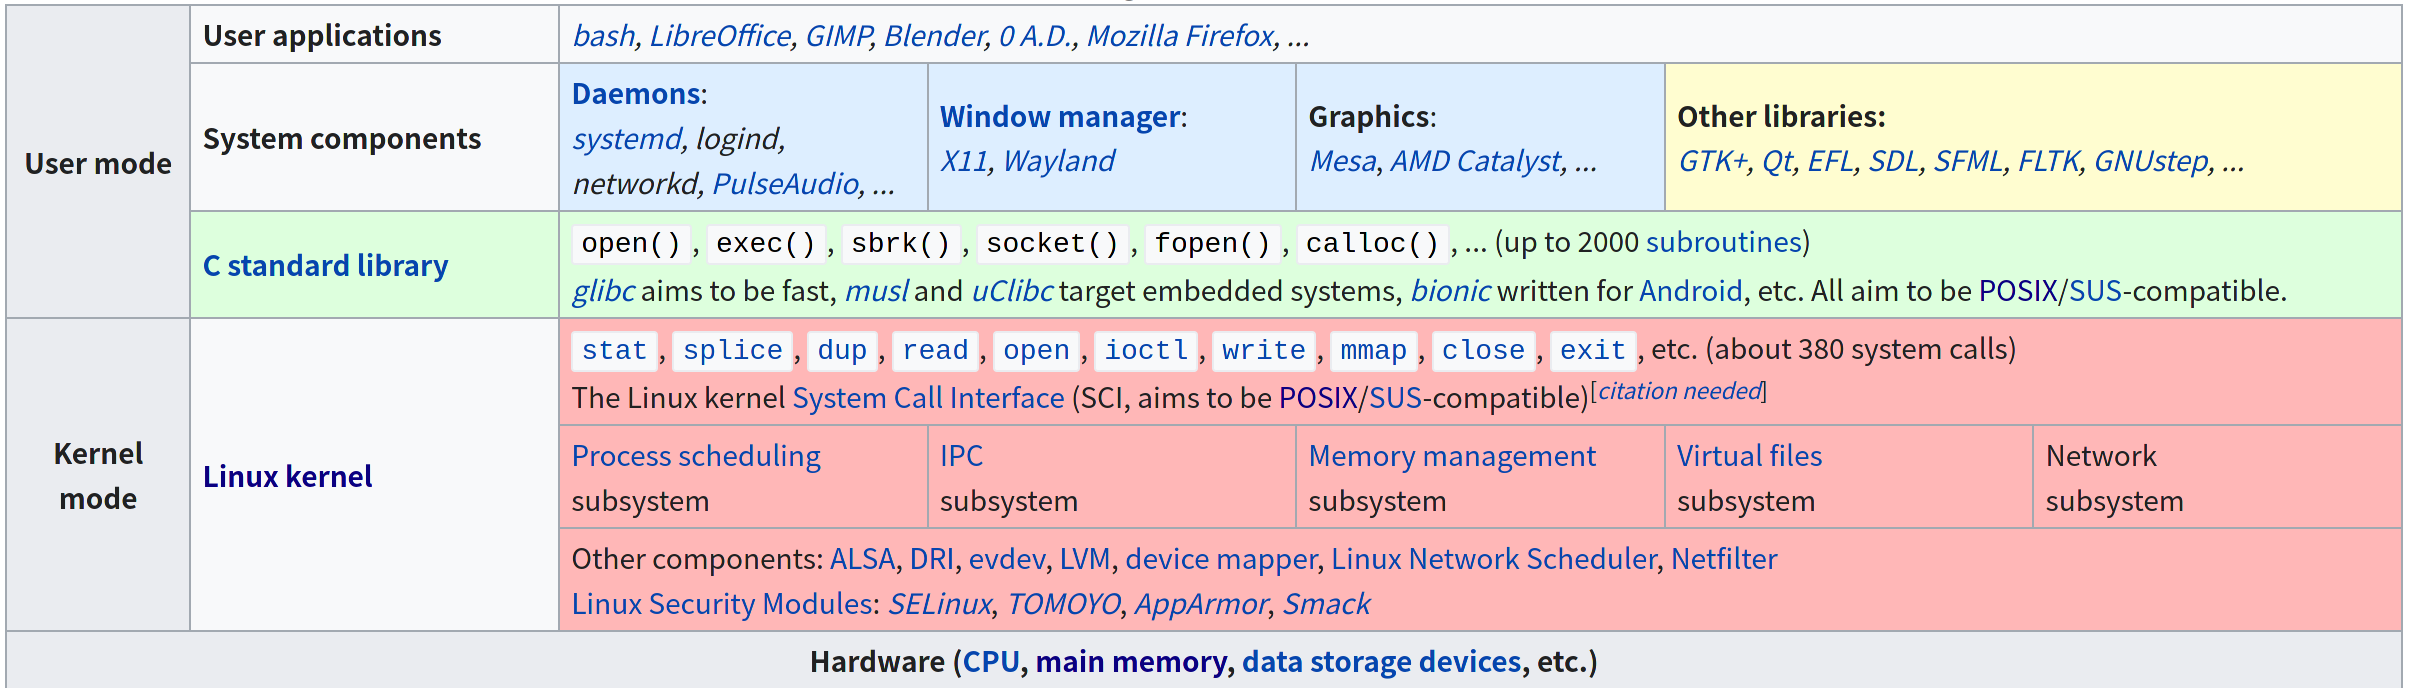
\includegraphics[center,scale=0.3]{linux-system.png}
\end{figure}

\vspace{2em}

\begin{center}
	\Large {\sout{\color{gray} 很无聊啊,这关我锤子事}}
\end{center}



\newpage
\section{GNU/Linux, for daily use}

\subsection*{为什么(现在)你会想要使用GNU/Linux}

\sout{在上一个section中,我们钦定GNU/Linux是适合日常办公学习;}\\
\sout{并且,可以在其上轻松搭建开发者,内容创作者,系统维护者所需的环境.}

\begin{itemize}[itemsep=0pt]
	\item 100 percent controllable
	\item 100 percent customizable
	\item embrace FOSS,community driven,decentralized
	\item for fun, for working efficiently, or for anything.
\end{itemize}


\subsection*{为什么(现在)你可以完全使用GNU/Linux}

\begin{itemize}[itemsep=0pt]
	\item 靠谱且稳定的kernel
	\item 完备的软件生态
	\item 友好、强大的社区+企业支持
\end{itemize}

已经是2021年.
不是那个canonical给全世界的网友邮寄光盘的年代; 
不是那个在slackware上面自己管理PHP,Apache http server,MySQL DB依赖的年代; 
不是那个每天kernel panic的年代; 
不是那个资料查不到,问人问不到,只能去邮件组里面被人喷,完全没有中文社区年代; 
不是那个分辨调节不了,天天屏幕撕裂的年代.\par

安装一个GNU/Linux发行版现在十分简单\footnote{gentoo这种需要compile the whole world的distro除外}; 
包管理器发展为强大的全系统维护工具,硬件驱动、字体、开发环境、GUI应用等等都可以无脑安装/更新/替换/卸载; 
kernel越来越稳定且高效,反倒是隔壁windows10天天蓝屏; 
桌面环境现在开箱即用,且定制性和集成度都有了巨大飞跃, 不少发行版可以做到无tty,无termial emulator使用; 
跨平台技术和基于web的技术 大势所趋, 专业内容生产创作或日常office办公,甚至影音娱乐, 都有了足够的软件支持; 
arch wiki/gentoo wiki多年积累,成为linux世界的comprehensive unofficial user manual+trouble shooting guide; 
有了github/gitlab等靠谱托管开发平台, 开发者 用户 维护者交流成本大幅下降; 
Linux使用的论坛不再冷清, 中文社区也有了足够的用户基础\footnote{我说的当然不是CSDN}.\\


\sout{好家伙,比某厂手机营销还离谱.}  我们不妨看一看网友们的使用经历, 以此, 初步检验现在完全使用GNU/Linux的可行性.\par
我在2020年初开始使用Linux环境工作, 在VirtualBox中运行manjaro, 并使用msys2模拟linux环境.  
到6月时,我确信自己积累了足够的经验, 于是把manjaro安装到了物理机上. 后来切换到了arch. 
遇到过一些小麻烦, 但都成功解决, 稳定使用至今\footnote{虽然目前没有出大问题,但定期备份还是要做的}.\par



\begin{center}
	\Large {\sout{\color{gray}为了学会开车,你并不需要了解内燃机工作原理和制造工艺}}
\end{center}

\newpage
\section{GNU/Linux, beginner's guide}

\subsection{尝鲜体验}

% 一些截图/视频/真机现场演示.
\emph{\color{red} TODO:个一些视频,真机现场演示.}

\subsection{安装与配置}

% 一个物理机安装视频.
\emph{\color{red}TODO:一个物理机安装视频.}

\subsection{获取帮助与支持}

\sout{讲解正确地搜索与提问方式. 或者说,出了锅怎么修}\\

我想trouble shooting中,最重要的是敢乱搞、敢提问的自信 以及 能全面认真地查阅资料的谦虚. 
当然, 也需要一些技术水准, 以解决那些前人未发现、未明确或为解决的问题.\par
必须说明的是,尽管arch wiki中文翻译做得不错, 中文社区现在初具规模, 使用英文仍是不可避免的.

\subsubsection*{step 1: 尝试复现问题,形成初步问题描述}

尝试复现问题的同时,也要尽量定位问题来源,确定问题的严重性.\par
清楚的问题描述和初步的定位,可以帮助你更有效的进行搜索,以了解潜在的解决方案或者进一步定位问题.\\



做问题复现请务必记住: 步骤最简,环境一致.\par
在这个过程中,你会对问题原因有初步认知, 比如是user space的问题还是kernel的问题, 是那个软件包/服务的问题, 是否与硬件平台相关等信息. 它们非常重要. \par
至于问题严重性的,新手常常会误判问题严重性.正如你所想,常常会高估问题严重性...
像kernel和fallback image同时挂了,没法boot; partial upgrade导致system break; grub无法引导等等,是很严重的问题,
而什么进不了桌面环境,屏幕撕裂了,某个配置不生效,某应用启动失败,是不那么严重的问题...\par



\subsubsection*{step 2: 尝试自己workaround}

当然,如果问题严重,别乱搞...转移工作空间的数据要紧.\par
具体而言: 用最新的arch iso做个live USB, boot到liveCD环境; 用外挂存储设备/网络连接拿走你的工作环境.  


\subsubsection*{step 3: (二手信息)查阅arch wiki/gentoo wiki}

事实上,多数你遇到的锅(不论什么发行版,什么软件环境,什么硬件平台),是被相当多的人发现,被前人准确定位,并找到了合适解决方案的.
这些信息被记录在各种神奇的地方, 当然arch wiki集中了most of them\par
arch wiki/gentoo wiki可以说无所不包, 别看顶着arch/gentoo发行版的名字, 实际上包含整个GNU/Linux生态的信息,甚至还有不少硬件相关的信息.
它们由用户群自发创建、自发维护,以及翻译. arch wiki是非常亲切的, 因为记录下那些信息的人和你我一样, 都是常规用户, 用户最清楚用户需要什么.

\subsubsection*{step 3: (二手信息)使用搜索引擎}

如果你不知道去wiki上面的什么词条找方案: 那么你应该先用step1中的信息进行搜索,以更好地定位问题,然后回到wiki.\par
如果认真仔细阅读了所有相关wiki词条,仍然没有解决问题: 那么你应当扩大信息搜集范围,利用搜索引擎找 user manual,blog,github issue,forum中的相关信息.\\


搜索引擎使用技巧...我懂得不多,只能给出一些零星的idea.
\begin{itemize}[itemsep=0pt]
	\item 使用关键词,而不是整句,防止SE的NLP错误理解问题; 
	\item 使用必须出现/必须不出某关键词的约束; 
	\item 使用and/or逻辑约束; 
	\item 使用site,title约束缩小范围; 
	\item 一次搜索很难解决问题, 往往需要分析查看结果,调整检索式,再次搜索,多次重复; 
	\item 注意语言的使用,多数情况下,英文资料最多最全, 但中国特供的产品/仅在中国流行的东西,显然要用中文, 必要时也可配合翻译工具搜索日文,德文等语种的资料.
\end{itemize}

\subsubsection*{step 3: 查官方文档}

有些过于细节的问题, 或者过于繁琐的问题, 需要在官方性质的文档中查阅. wiki不会搬运这种东西.

\subsubsection*{step 4: 问人}

描述问题,给出环境和复现方式; 描述你查阅到的相关信息,和进行的尝试. 注意排版...有大段log/code可以使用ubuntu pastebin.\par
然后,耐心等,耐心和愿意提供帮助者进一步交流情况.\par
并且记住,没有人有义务帮助你; 以及,你时常会遇到当前不存在较好解决方案的问题,甚至是目前没有明确原因的问题.\\

为什么人们(尤其是开发者和维护者)讨厌伸手党? 因为它们比起数量增长的推广和扩张, 更关心功能改进、问题修复、稳定性提升和技术创新的质量提升. 而复制粘贴解决方案给伸手党, 最多是拉拢一些不可能成长为贡献者的初级用户.\\

\subsubsection*{step 5: 自己动手,丰衣足食}

到了这里, 你可能进入无人区了. 你遇到的问题, 可能是未发现/未明确/未解决状态. 具体是那种得去上游找.\par
请首先想办法workaround, 以继续正常工作. 比如``问题不大,可以忍'',``从某个路径下、在启动某个服务之后运行它,就不会有问题'',``写一个脚本wrap它,hook一些syscall做些特殊处理''.\par
之后找上游\footnote{指软件开发者 / 硬件、驱动、固件提供商}看看问题是属于那种情况: 
\begin{enumerate}[itemsep=0pt]
	\item 已经修复,尚未跟进
	\item 已经被发现,尚未修复
	\item 没有被遇到过/没有被报告
\end{enumerate}
1 请联系发行版的软件包打包者.\\
2 可以汇报问题再现的情况 \sout{其实就是催更}.\\
3 请上报给开发者. 可能是 github/gitlab发issue, bugzilla汇报, 也可能是其他渠道,比如trac ticket. 具体如何上报问题一般会在user manual / how to contribute 文档中描述.\\
当然如果您能写个patch修锅,或者fork出去修掉再pr/mr回去最好.  


\subsubsection*{step $\infty$: 记录与分享}

我们进行trouble shooting用到的资料, 都是其他用户无偿分享的. 
所以做为回报, 我们也要做对等的记录与分享.\par
比如写一篇对搜索引擎友好的blog, 让其他人在搜索时, 能够少走弯路.  
或是帮助完善arch wiki, 使它更加完备, 维持其``a comprehensive unofficial guide for GNU/Linux''的作用. 



\newpage
\subsection{软件生态}

更全面的介绍见 arch wiki的两个词条\href{https://wiki.archlinux.org/index.php/List_of_applications}{1},\href{https://wiki.archlinux.org/index.php/General_recommendations}{2}.\par
以及桌面环境配套应用\href{https://userbase.kde.org/Applications}{KDE} \href{https://wiki.gnome.org/Apps}{Gnome}.

\begin{itemize}[itemsep=0pt]
	\item 选择KDE plasma5或者Gnome3获得完整的桌面环境.\\ 也可以用精简的i3,sway,bspwm等窗口管理器 
	\item 想要安装新软件,却不会用包管理器的CLI?\\ 试试KDE下的discover或者Gnome下的Gnome software center.
	\item 都用上GNU/Linux,总不能还 微软雅黑+时代新罗马 吧\footnote{MS font可以搞,但是没必要}.\\ 试试google noto,adobe source等开源字体吧.\\ 在KDE/Gnome中配置字体非常容易,不需要手写fontconfig.
	\item 安装fcitx5-im组(包含fcitx5,fcitx5-qt,fcitx5-gtk,fcitx5-configtool),\\ 之后按照wiki指示安装你喜欢的输入法并进行配置.
	\item 浏览器当然选择firefox.\footnote{chrome,chromnium,edge,brave可选,但是我不会推荐它}
	\item 什么时候有SIST seminar?需要给老板发邮件?outlook没了?\\ 安装kmail/evolution获得邮件与日程管理\footnote{evolution支持exchange协议}
	\item 聊天社交使用 telegram,IRC,tox. 腾讯家的wechat,qq比较难搞.
	\item 安装LibreOffice / OpenOffice代替MS office.\footnote{WPS office有原生Linux版,MS office可以通过wine完美运行,但是我不会推荐它} 没了拼写纠错?安装aspell,hunspell和语言包就行啦.
	\item 使用okular阅读多种文档; 配合pandoc进行文档格式转换.
	\item 安装vlc获得多媒体支持\footnote{常规的codec,ffmpeg等依赖不需要手动安装,会被包管理器安排好},甚至还有你熟悉的网易云音乐\\  图片/相册管理 使用EOE/Gwenview.
	\item 懒得自己做数学题? sagemath提供完整数学环境,octave替代MATLAB core; 还有你熟悉的scipy以及R.
	\item 备份和同步 timeshift,syncthing. 当然也有dropbox,onedrive,google drive.
	\item XX手机助手没了? 使用scrcpy + kde-connect来融移动平台和桌面平台.
	\item Wine+Qemu(with KVM)解决Linux无法使用的软件 \sout{腾讯全家桶;steam;垃圾multisim}.
	\item 编辑器当然用vim/Emacs. 懒得自己配置用spaceVim/spaceEmacs.\\ 也可以试试你们熟悉的VS code与typora.
	\item 有专业需求? 是一名软件开发者,内容创作者,或是科研人员.\\ 参考arch wiki list of applications,你们熟悉的环境,这里都有.
	\item 跨过长城,走向世界? 你熟悉的暗影袜子/第二光线都可以轻松搭建.
	\item \sout{夹带私货} 一些有趣的TUI/CLI应用,轻松帮你工作效率翻倍: 
		\begin{itemize}[itemsep=0pt]
			\item 基础工具: core-utils,gnu-toolchain,git,tmux,openssh,vim...
			\item 包管理器: arch系使用pacman;ubuntu使用apt;RPM系使用dnf.
			\item init系统: systemd或者open rc,进行服务管理/定时任务/hook脚本.
			\item fish,zsh: 更友好的shell,提供补全、纠错、快速跳转等特性,吊打bash.\\ 对于脚本编程,我推荐python而非任何一种shell.
			\item nmcli,iwctl: network manager和iwd的前端,快速管理网络连接.
			\item tldr\footnote{too long, don't read. 或者说 太长不看}: 帮助文档速查,部分代替man pages.
			\item rsync: 远程同步工具. 还可以用vim+rsync干掉VSC remote dev.
			\item ranger,broot: TUI文件管理器.
			\item FuzzyFileFinder(fzf)+theSilverSearch(ag)+ripgrep(rg)
			\item curl: 访问HTTP/FTP/redis/memcached.
			\item aria2: 多线程下载器,支持断点续传.
			\item proxychains: 环境变量http\_proxy,socks5\_proxy不生效,怎么办.
			\item pandoc: 构建不同文档格式为顶点的完全图
			\item aspell: 拼写检查工具.
			\item rofi: 最棒的app launcher.
		\end{itemize}
\end{itemize}

\newpage
\section{random thoughts on FOSS}

我不想讨论fres software和open source的区别, 不想讲解RMS和FSF的执念, 也不想画大饼构想totally free and open的未来.\par
我想,当前人类还未有物质极大丰富而走向共产主义, 自由软件运动也仅仅是初级阶段. 不如现实一点, 实用意义大于意识形态, 只要我们心中还有自由并且用实际行动促进开放, FOSS就不会死去.


\subsection{FOSS, not only open source}

继续之前,先来谈谈自由软件和开源软件\par

首先是自由软件,GNU定义的free software: respects users' four essential freedoms.
其着眼点在于用户的自由权利.

\begin{enumerate}
	\item[0] The freedom to run the program as you wish, for any purpose.
	\item The freedom to study how the program works, and change it so it does your computing as you wish.
	\item The freedom to redistribute copies so you can help others.
	\item The freedom to distribute copies of your modified versions to others.\\ By doing this you can give the whole community a chance to benefit from your changes. 
\end{enumerate}

而开源软件,要求使用open source licenses\footnote{例如GPL,Apache license,MIT Lincense}授权.
任何人都可以获得开源软件,它注重软件透明可信和社区协作的可能性.


\subsection{FOSS, community driven}

什么是社区? 就是用户+开发者+维护者的人群与信息交流公开渠道+组织\footnote{我们还是不能太理想化,现实一点, 这里不可避免地会有企业巨头和资本的影响.\\ 看看kernel代码贡献来源就知道了}.\par
GNU/Linux的社区乃至整个FOSS世界的特点, 我认为有这样三点: 自由,开放,对等.

\subsection{FOSS, contributing}


社区特点中的对等,是指用户,开发者,维护者这三个角色没有实质区别.\par
我们应当意识到FOSS来之不易,且其发展面临压力, 所以用户应当做开发者和维护者的工作. 
而此外,``使用''本身也可以是一种贡献\par


\begin{itemize}[itemsep=0pt]
\item 仍然有人在使用他们的软件, 他们的软件将来也会有更多的用户.\\
	用户是开发者和维护者继续贡献的动力来源之一.
\item 用户在使用中会发现bug,定位问题,并且可能辅助修复; 使用者也会提供强化功能和优化体验的建议甚至解决方案.\\
	用户是FOSS进步的来源之一.
\end{itemize}


\newpage
\appendix
\section{reference \& resources}

\subsection*{本次分享的参考资料}
\begin{itemize}[itemsep=0pt]
	\item \href{https://101.lug.ustc.edu.cn/}{USTC linux101}
	\item \href{https://www.gnu.org/}{GNU official site}
	\item \href{https://opensource.com/resources/what-open-source}{OpenSourceInitiative}
	\item \href{https://creativecommons.org/licenses/}{CreativeCommons lincense}
	\item \href{https://distrowatch.com/}{distrowatch}
	\item wikipedia: \href{https://en.wikipedia.org/wiki/Unix}{UNIX},\href{https://en.wikipedia.org/wiki/Linux}{Linux}
\end{itemize}

\subsection*{可以随便看看,找找有趣东西的视频}

\begin{itemize}[itemsep=0pt]
	\item \href{https://space.bilibili.com/13081489}{拉我入坑的TheCW at bilibili}
	\item \href{https://space.bilibili.com/40420441}{Houge Langley的乐享linux生活/linux头脑风暴系列视频}
	\item \href{https://space.bilibili.com/327222212}{brain的linux体验视频}
\end{itemize}

\subsection*{获取发行版的ISO镜像}

\begin{itemize}[itemsep=0pt]
	\item 各种发行版的官网: \href{https://cn.ubuntu.com/download}{ubuntu},\href{https://manjaro.org/get-manjaro/}{manjaro},\href{https://getfedora.org/}{fedora},\href{https://pop.system76.com/}{Pop!\_OS}...
	\item 国内的镜像、反代站: \href{https://mirrors.tuna.tsinghua.edu.cn/}{清华的Tuna mirrors},\href{http://mirrors.ustc.edu.cn/}{中科大镜像站},\href{https://mirrors.geekpie.club/help/}{张江理工镜像站}
\end{itemize}

\subsection*{虚拟机, POSIX兼容层, win32兼容层}
\begin{itemize}[itemsep=0pt]
	\item Qemu; VirtualBox
	\item \sout{Cygwin}\, msys2\footnote{msys2早就可以完全取代Cygwin并且比其做得更好了},WSL, wine
\end{itemize}

\subsection*{出了问题去哪里问}
\begin{enumerate}
	\item ask your self / try to fix it by yourself
	\item bing/google/duckduckgo search engine
	\item Arch Linux wiki; \href{https://wiki.archlinux.org/index.php/Frequently_asked_questions}{arch wiki:FAQ}
	\item the software's official documentation; man page; tldr pages; github.
	\item ArchLinux forum\& Unix Stackexchange\& Ask Ubuntu\& Stack Overflow ;\quad telegram群组,IRC 群聊,邮件组.
\end{enumerate}

\end{document}


